\newpage
\section{Praktische Umsetzung}\label{sec_praktische_umsetzung}

In der praktischen Umsetzung werden die Grundlagen auf den Anwendungsfall angewendet.
Als Einführung in den praktischen Teil wird zunächst das Zielbild der Projektarbeit im Detail erläutert.
Es folgen die Bildklassifizierung und die Umsetzung der \acf{NER}.

\begin{figure}[H]
	\caption{Zielbild des Consulting-Projekts}\label{fig:zielbild}
	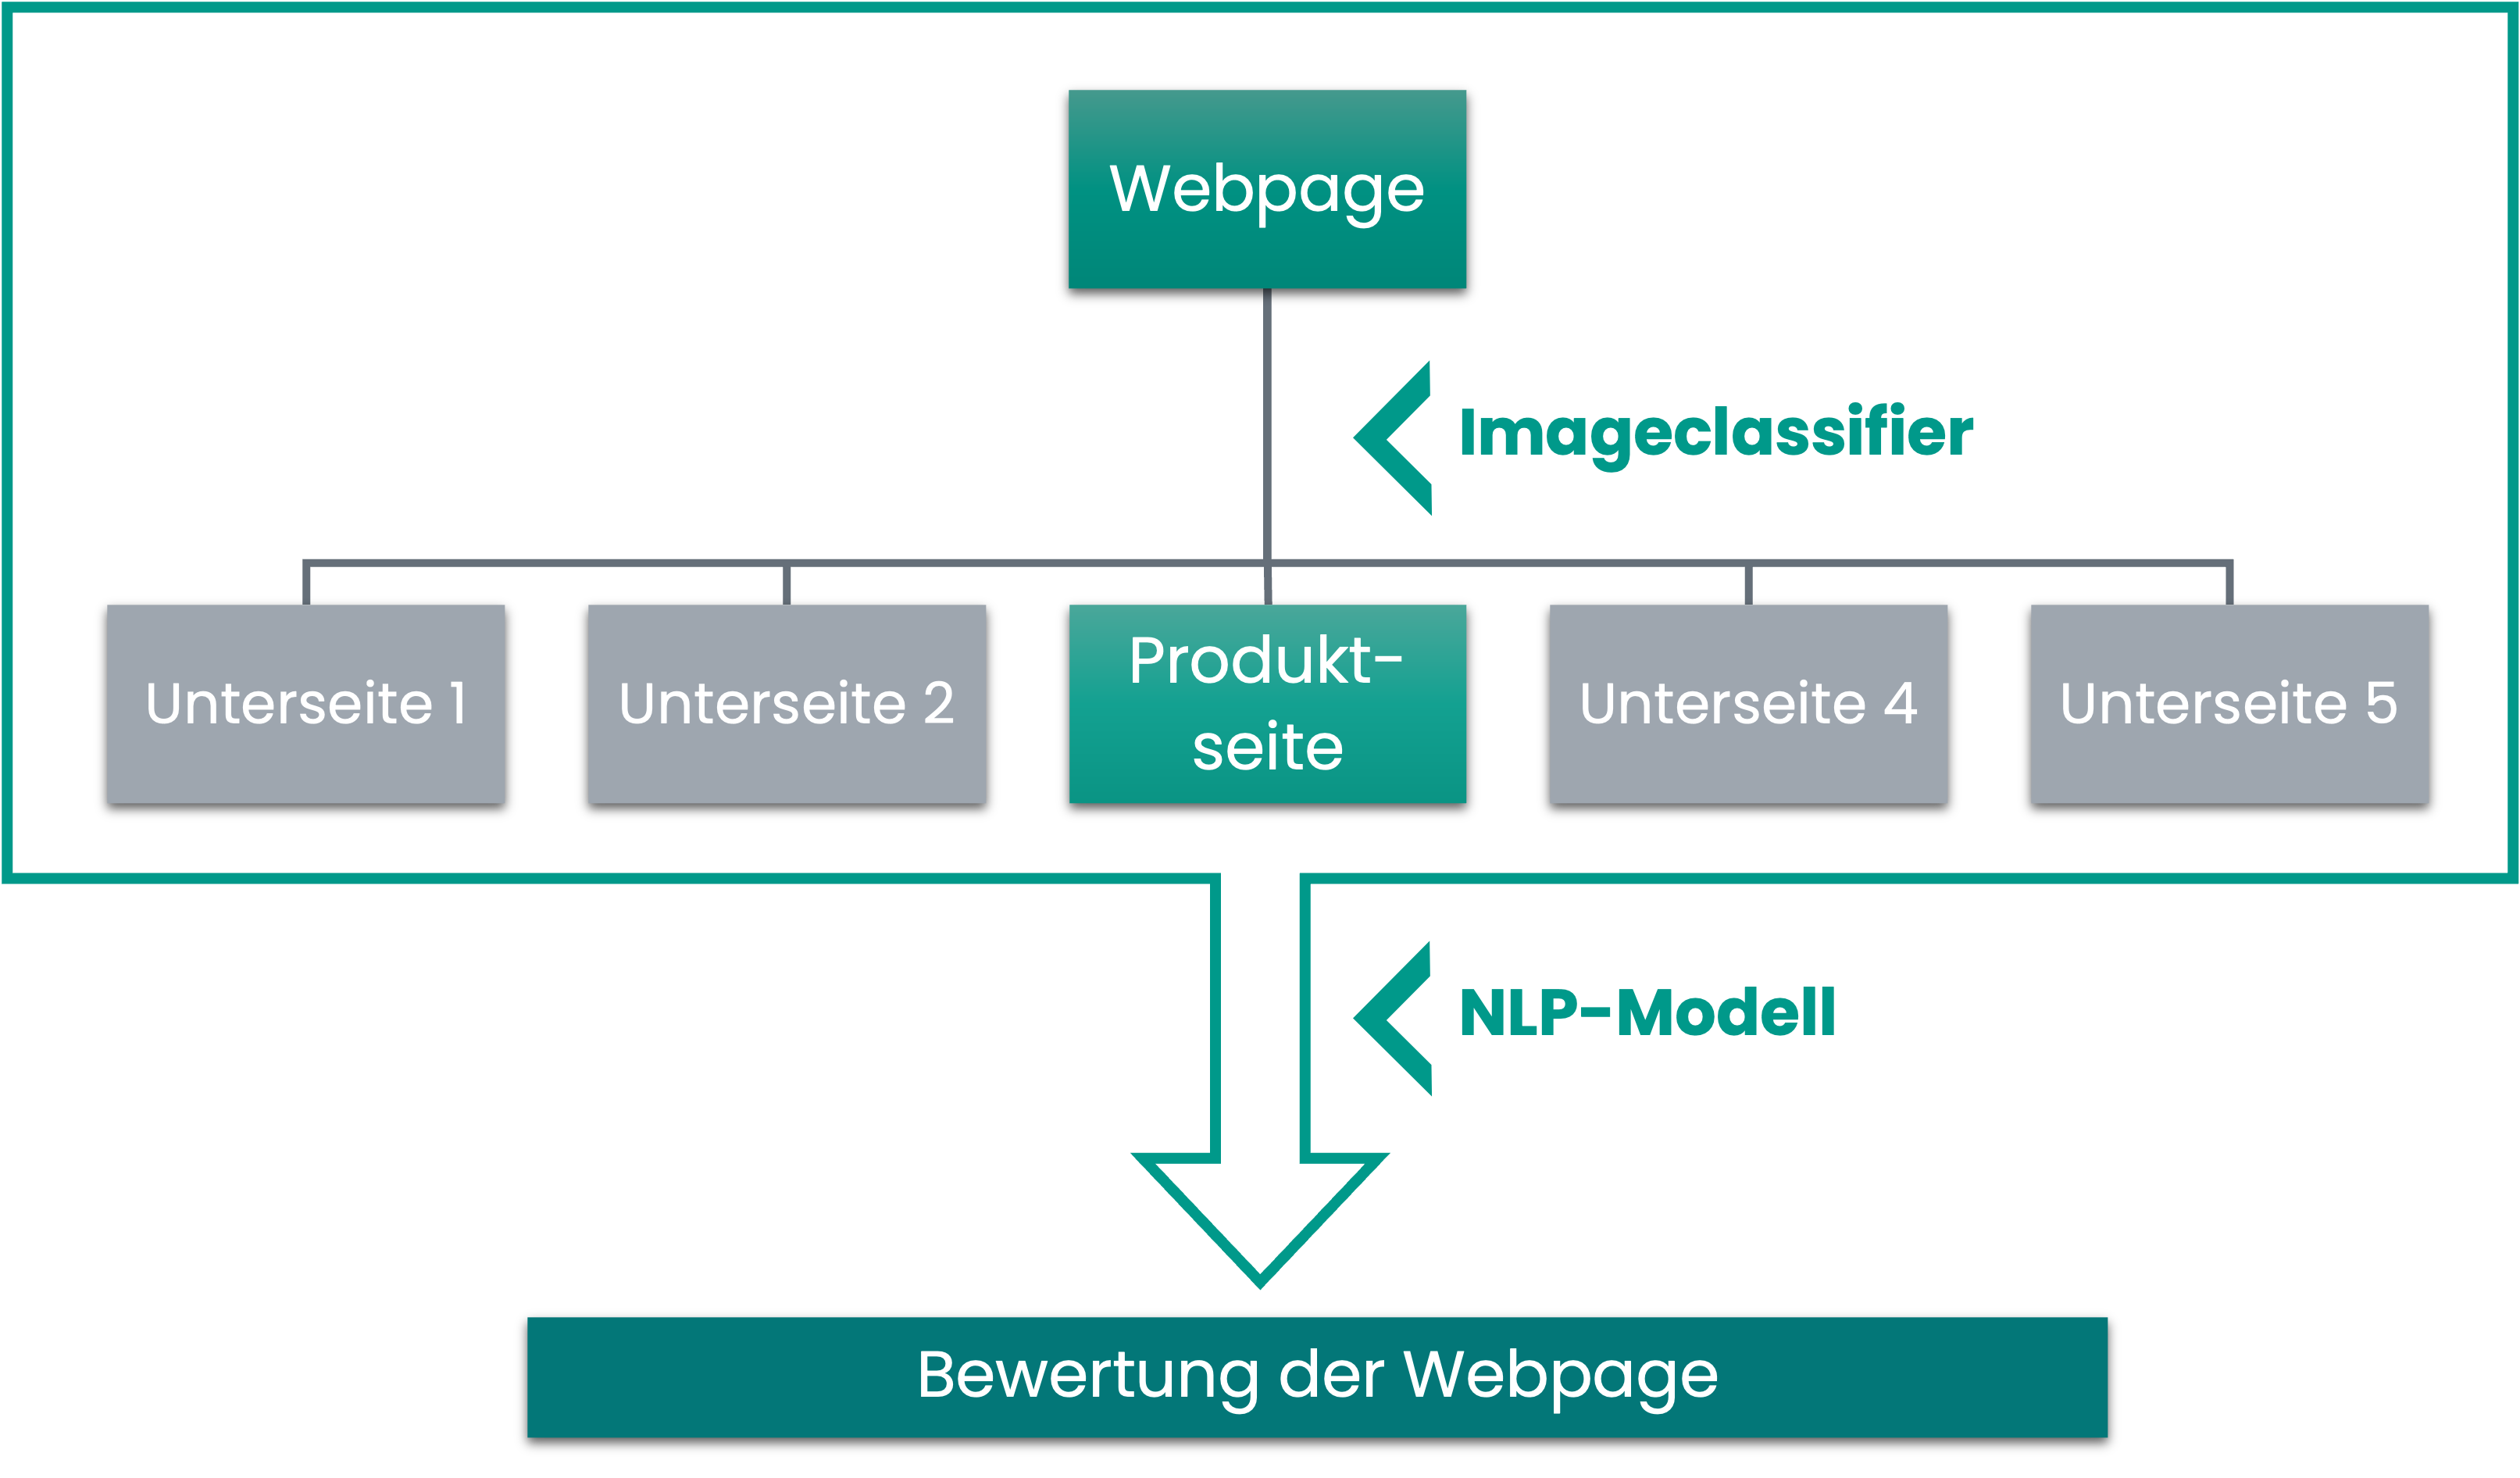
\includegraphics[width=0.9\textwidth]{zielbild.png}
	\\
	Quelle: Eigene Darstellung
\end{figure}

Um den OSMI-Index zu optimieren und zu automatisieren, wurde die in Abbildung~\ref{fig:zielbild} dargestellte Pipeline aufgestellt, mithilfe dessen
eine Website in Bezug auf den OSMI verarbeitet wird.
Der erste Schritt stellt dabei eine Vorverarbeitung der zu analysierenden Website dar, indem ein Image Classifier die Haupt- und Unterseiten der Website in
Produkt- und Nicht-Produktseiten unterteilt.
Dies ist aus Sicht der Autoren dieser Hausarbeit ein essenzieller Schritt, da so sichergestellt wird, dass die Bewertung des OSMI-Index lediglich auf Basis
der relevanten URLs vorgenommen wird.
Im darauf folgenden Schritt wird auf die textlichen Inhalte der relevanten Produktseiten ein \ac{NLP}-Modell angewendet, welches die Entitäten des OSMI-Index erkennt und auszählt.
Im abschließenden Schritt werden die Ergebnisse der Website-Analyse im Rahmen eines Dashboards visualisiert.
Nachfolgend wird die Umsetzung der soeben beschriebenen Schritte im Detail beschrieben und erläutert.

\subsection{Datenvorbereitung}

Sowohl in der Literatur als auch in bereits etablierten, gut entwickelten und veröffentlichten Modellen ist das Gebiet
des Sensory Marketings sehr rar vertreten.
Das bedeutet auch, dass im Hinblick auf den jüngst publizierten \ac{OSMI}-Index ebenfalls bisher wenig technische Entwicklungen
vorgenommen worden sind.
Zwar existieren in der Literatur diverse NLP-Modelle wie beispielsweise das Spacy-Modell~\footcite[\vglf][]{spacy2017} oder der sogenannte BERT~\footcite[\vglf][]{devlin2018}
und von beiden erwähnten Modellen Spezialisierungen wie beispielsweise SciSpacy, BioBERT, ESG-BERT, allerdings ist
bisher kein \ac{NLP}-Modell auf Marketingkontexte trainiert und publiziert worden. Daher besteht die Notwendigkeit zur Entwicklung eines
eigenen Modells im Kontext des Consulting-Auftrags.
Um im Vorfeld der Website-Bewertung jedoch lediglich nur die relevanten URLs mit Produktinhalt zu selektieren, wurde für den zu
entwickelnden Image Classifier ebenfalls ein von Grund auf neu zu entwickelndes Modell benötigt, da es innerhalb der Literatur
bislang kein derartig existierendes Modell publiziert wurde auf das zurückgegriffen werden konnte.

Die Trainingsdaten wurden mithilfe von Doccano generiert.
Doccano~\footcite[\vglf][]{doccano-2018} ist eine Open Source Software, welche zur Annotation von Text und Bilddaten entwickelt wurde.
Mit diesem Instrument ist es also möglich Textpassagen und Bilder hochzuladen und Annotationen vorzunehmen, um Daten zur
Entwicklung von Aufträgen wie \acl{NER}, Textzusammenfassungen, Sentimentanalysen, Image Classification, etc.\ zu generieren.

Im Rahmen des Consulting-Projekts wurden zwei Doccano-Projekte gestartet.
Ein Projekt wurde für das Annotieren von Textpassagen zur Entwicklung eines \acl{NER} Modells erstellt.
Im zweiten Projekt wurden Screenshots von Produktseiten und Nicht-Produktseiten annotiert um ein Classification Modell erstellen zu können.

Die Textpassagen, die annotiert wurden, sind im Rahmen des Consulting-Projekts zur Verfügung gestellt worden und entstammen
Webscraping-Ergebnissen von Vorgängerprojekten.
Hier wurden die fünf Sinne \textit{Sight}, \textit{Smell}, \textit{Sound}, \textit{Taste} und \textit{Touch} als Label festgelegt, da dies die Entitäten sind die später auch für den OSMI nach Hamacher notwendig sind.

Abbildung~\ref{fig:annotation_ner} stellt ein Balkendiagramm über den Annotationsstand dar, das die Häufigkeit der einzelnen Labels aufzeigt. Diese Verteilung der Daten bildet die Basis auf der das Modell zur Erkennung von Entitäten trainiert wurde.
Es ist zu erkennen, dass die Entität \textit{Sight} am häufigsten annotiert worden ist, während die Trainings- und Testdaten für
die Entitäten \textit{Smell}, \textit{Sound} und \textit{Taste} kaum vertreten sind.
\begin{figure}[H]
	\caption{Annotationsstand Textlabeling}\label{fig:annotation_ner}
	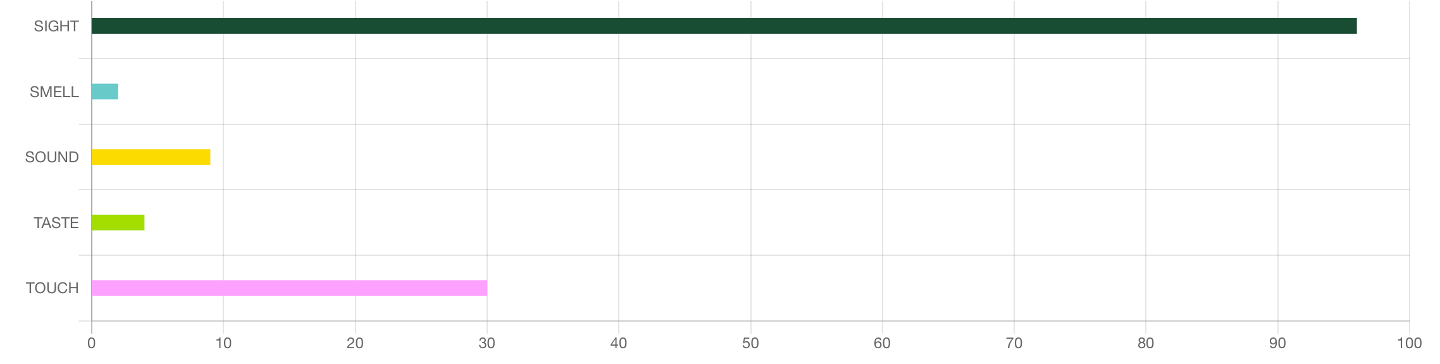
\includegraphics[width=0.9\textwidth]{annotationen_ner.png}
	\\
	Quelle: Eigene Darstellung
\end{figure}

Die zu annotierenden Bilddaten von Produkt- und Nicht-Produktseiten wurden im Rahmen des behandelten Projektes erneut gesammelt (siehe auch Abschnitt \ref{subsubsec_class_datenverarbeitung}).
Abbildung~\ref{fig:annotation_imgclf} zeigt, dass zur Modellentwicklung für den Image Classifier eine annähernde Gleichverteilung zwischen Produkt-
und Nicht-Produktseiten zugrunde gelegt werden konnte.
Der Gesamtdatensatz beläuft sich auf rund 500 annotierten Bildern von Homepages.
\begin{figure}[H]
	\caption{Annotationsstand Textlabeling}\label{fig:annotation_imgclf}
	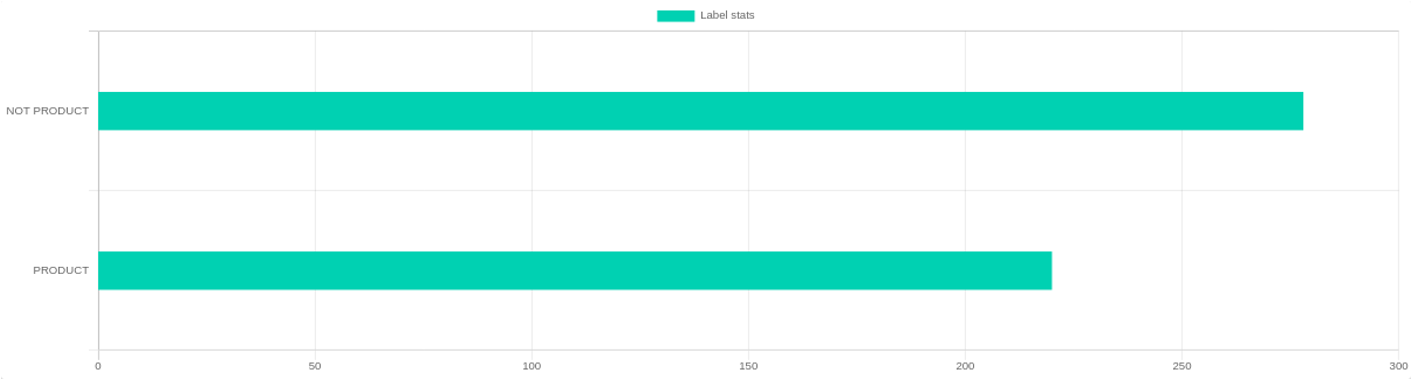
\includegraphics[width=0.9\textwidth]{annotationen_imgclf.png}
	\\
	\textit{Quelle: Eigene Darstellung}
\end{figure}


\subsection{Modellentwicklung}

\subsubsection{Image Classification Modell}
% \textcolor{red}{
% 	\begin{itemize}
% 		\item Gewichtung der Indikatoren wird im \ac{OSMI} nicht vorgenommen, weil nicht zweifelsfrei zu
% 		argumentieren welcher mehr oder weniger bewertet wird (bisher keine Forschungsarbeiten
% 		dazu)
% 		\item Indikatoren werden einzeln bewertet \& letztendlich fünf Parameter zw. 0 \& 1 liegen vor.
% 		Daraus ergibt sich Gesamt-Index (ohne Gewichtung, arithmetischer Durchschnitt) für jede
% 		Webseite > auch zw. 0 \& 1 und ist dann der \ac{OSMI}-Index
% 		\item Je näher der \ac{OSMI} an einer 1, desto erfolgreicher spricht die Webseite die Sensorik an. Wert
% 		nahe 0 erhält wichtige Elemente entsprechend nicht \& erfüllt die Indikatoren nicht
% 		\item BSP eines \ac{OSMI}-Indexes: Bild einfügen aus der Masterarbeit mymuesli.de oder so
% 	\end{itemize}
% }

% \textcolor{red}{
% möglicher Aufbau:
% \begin{itemize}
% 	\item Bildklassifizierung
% 	\begin{itemize}
% 		\item Datenset
% 		\item Umsetzung
% 	\end{itemize}
% 	\item NER
% 	\begin{itemize}
% 		\item Datenset
% 		\item Umsetzung
% 	\end{itemize}
% 	\item Zusammenführung
% 	\item Consultingteil
% \end{itemize}
% }

\subsection{Klassifizierung von Webseiten}\label{subsec_klassifierung_websites}
Es soll ein Modell entwickelt werden, dass in der Lage ist zwischen Produkt und nicht-Produktwebseiten zu unterscheiden.
Wie Kapitel~\ref{sec_grundlagen_image_classification} deutlich geworden ist, kann dies von Klassifizierungsmodellen geleistet werden.
Im Folgenden wird das Vorgehen mit den Schritten der Datenerhebung (\ref{subsubsec_class_datenerhebung}), der Datenverarbeitung (\ref{subsubsec_class_datenverarbeitung}) und des Modelltrainings (\ref{subsubsec_class_training}) näher beschrieben.

\subsubsection{Datenerhebung}\label{subsubsec_class_datenerhebung}
Aus vergangenen Arbeiten von Studierenden steht bereits eine Datengrundlage zur Verfügung mit Textauszügen, dem HTML Quelltext und heruntergeladenen Bildern von Unternehmenswebseiten.
Grundsätzlich sind dies die Elemente, die die semantischen und inhaltlichen Informationen der Webseite beinhalten, allerdings fehlen zwei für das äußere Erscheinungsbild der Webseite notwendige Elemente:
Javascript, das für das dynamische Verhalten der Webseite verantwortlich ist und CSS, das für das Styling der HTML-Elemente verwendet wird.
Wären diese Elemente vorhanden, so könnten sie - insofern sie in der richtigen Struktur vorliegen - dafür verwendet werden auch nachträglich, offline das Erscheinungsbild der Webseiten zu reproduzieren.

Vor diesem Hintergrund konnten daher die bereits gesammelten Daten nicht verwendet werden und es war notwendig eigene Screenshots mit einem Webscrawler zu erstellen.
Für die Klassifizierung werden jedoch Bilder beziehungsweise Screenshots benötigt, die die gerenderte, visuelle Struktur der Webseite erfassen.
Dies ist in den bestehenden Daten nicht gegeben und machte daher eine erneute Erhebung notwendig.

Für diesen Zweck wurde zunächst ein Webcrawler auf Basis von Scrapy~\footcite[\vglf][]{zotero-328} erstellt,\footcite[\vglf][]{ostkamp2022a} der alle in der Vergangenheit gescrapten Webseiten aufruft und einen Screenshot der jeweiligen Seite erstellt.
Auf diese Weise wurden circa 10.000 Bilder gesammelt, die als Eingangsdaten für das Modell verwendet werden können.

Zwei Probleme sind bei der Datenerhebung zutage getreten.
Webseiten sind - gerade im Bereich von Unternehmen und Marketing - stetigen Veränderungen ausgesetzt. Dies zeigte sich auch in der erneuten Erfassung nach über zwei Jahren, da für einige Urls die Webseite nicht mehr verfügbar war (siehe auch Abbildung~\ref{fig:doccano_products}).
Ein zweiter Aspekt der dynamischen Natur von Webseiten ist die Veränderung des Inhalts, der sich rückwirkend nicht so einfach feststellen lässt wie eine 404 Status Page, der dennoch aber nicht ausgeschlossen werden kann.

Das zweite wesentliche Problem war technischer Natur und bezog sich auf die Ladezeiten der Webseiten. In einigen Fällen ist es vorgekommen, dass auch nach einer Wartezeit von 3 Sekunden, noch nicht alle Elemente der Webseite - insbesondere Bilder - geladen waren.
Die gewählte Wartezeit sollte vor dem Hintergrund der Internetverbindung und der Ladezeit typischer Webseiten (Zitat) eigentlicht ausreichend sein, um eine vollständig geladene Seite zu erfassen.
Die Autoren haben darauf verzichtet sie weiter zu erhöhen, da auch mit der gewählten Zeit bei 10000 Seiten ein Durchgang bereits 8 Stunden dauert und jede weitere Sekunde eine Verlängerun g von 3 Stunden bedeutet.

\begin{figure}[H]
    \centering
    \caption[]{Bildklassifizierung in Doccano}
	\label{fig:doccano_products}
    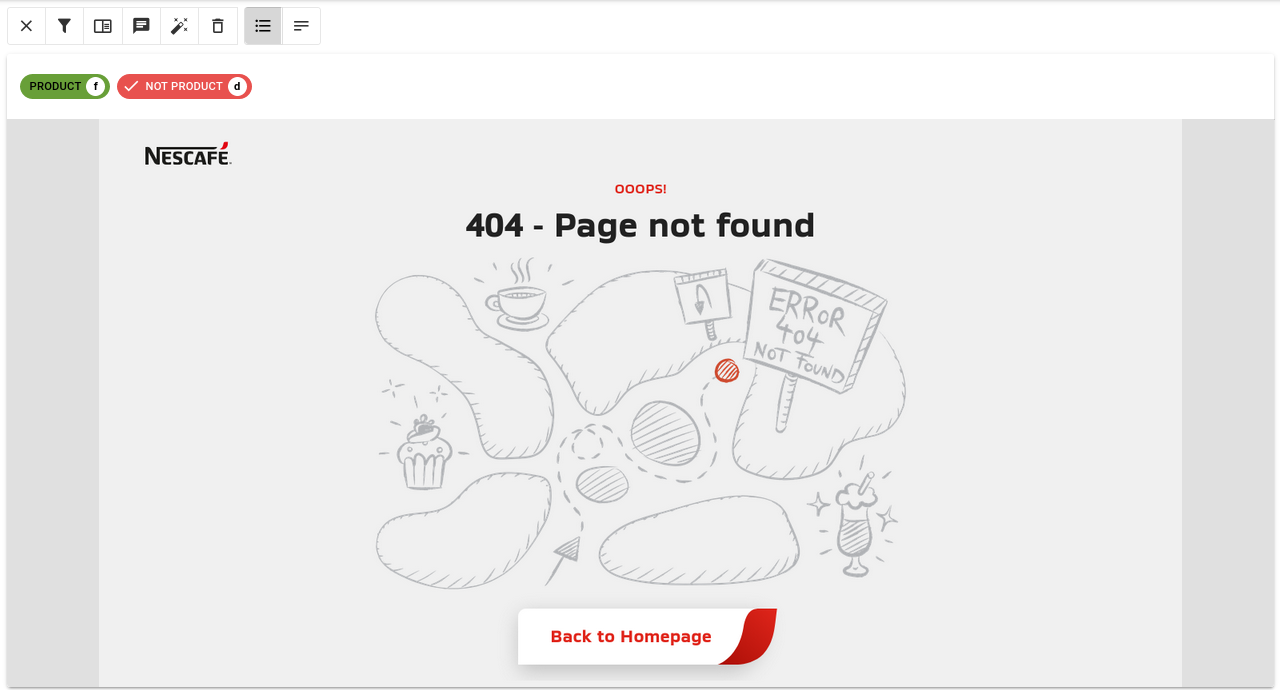
\includegraphics[width=1\textwidth]{doccano_product_annotation.png}
	\\
	\textit{Quelle: Eigene Darstellung}
\end{figure}
Da es sich bei der Klassifizierung um eine Supervised Learning Methode handelt, müssen die Daten daraufhin den Kategorien \textit{Product} und \textit{Non Product} zugeordnet werden.
Dafür werden die Daten in die Annotationssoftware Doccano~\footcite[\vglf][]{doccano-2018} geladen und dann, wie in Abbildung~\ref{fig:doccano_products} dargestellt, den Kategorien zugeordnet.

\subsubsection{Datenverarbeitung}\label{subsubsec_class_datenverarbeitung}
Im Schritt der Datenverarbeitung werden die Eingangsdaten in eine Form gebracht, in der sie für das Training des Modells verwendet werden können.
Dazu werden die Bilder anhand des Exports der Annotationen aus Doccano in den Labeln gleichnamige Ordner verschoben.

Da die Screenshots als \textit{.png} Bilder vorliegen, verfügen sie über einen Alpha-Channel der für die Verwendung im Modell hinderlich ist.
Aus diesem Grund wurde dieser in einem weiteren Schritt entfernt.
Darüber hinaus werden die Bilder im ersten Layer des Modells auf eine Größe von 224x224 Pixeln herunterskaliert, was eine gängige Größe für \aclp{CNN} darstellt.\footcite[\vglf][\pagef 79]{ghosh2019}


\subsubsection{Training des Modells}\label{subsubsec_class_training}
Nachdem die Daten, wie in Kapitel~\ref{subsubsec_class_datenverarbeitung} beschrieben, verarbeitet wurden, können Sie im weiteren Verlauf für das Training eines Modells verwendet werden.
Dazu wurden die Daten wie im Deep Learning üblich, in Train und Validation Sets aufgeteilt um einen späteren Vergleich auf unbekannten Daten zu ermöglichen.
Aufgrund der geringen Menge der Eingangsdaten wurde \textit{Data Augmentation} verwendet um durch leichte Mutationen der Bilder wie etwa Zooming oder eine vertikale Spiegelung Overfitting zu reduzieren.
\begin{figure}[H]
    \centering
    \begin{subfigure}[b]{0.49\textwidth}
        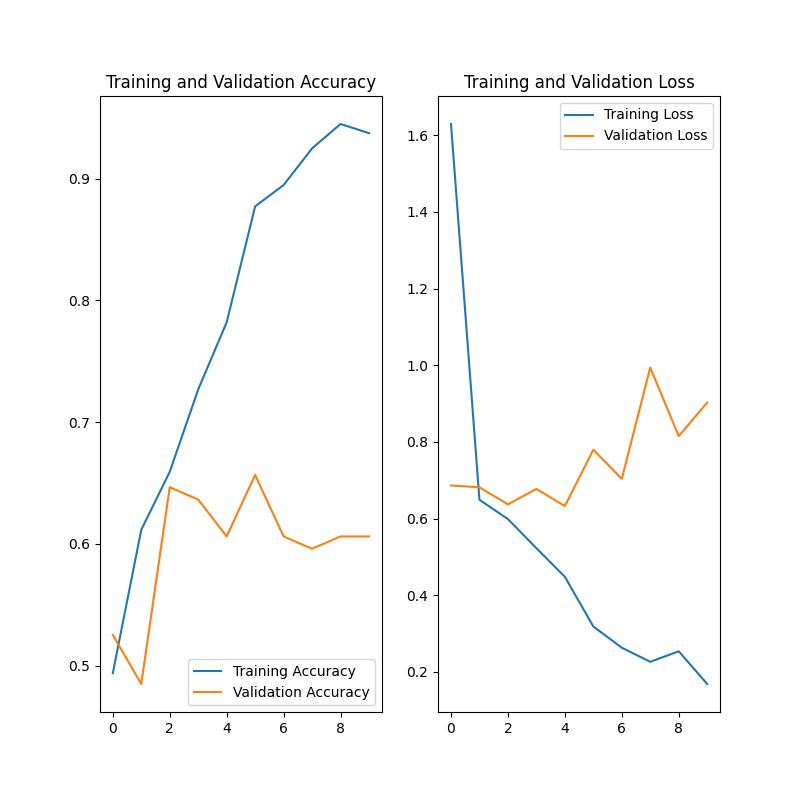
\includegraphics[width=\textwidth]{abbildungen/acc_train_val.png}
        \caption{Ohne Data Augmentation}\label{fig:metricsTrainWOAugmentation}
    \end{subfigure}
    \begin{subfigure}[b]{0.49\textwidth}
        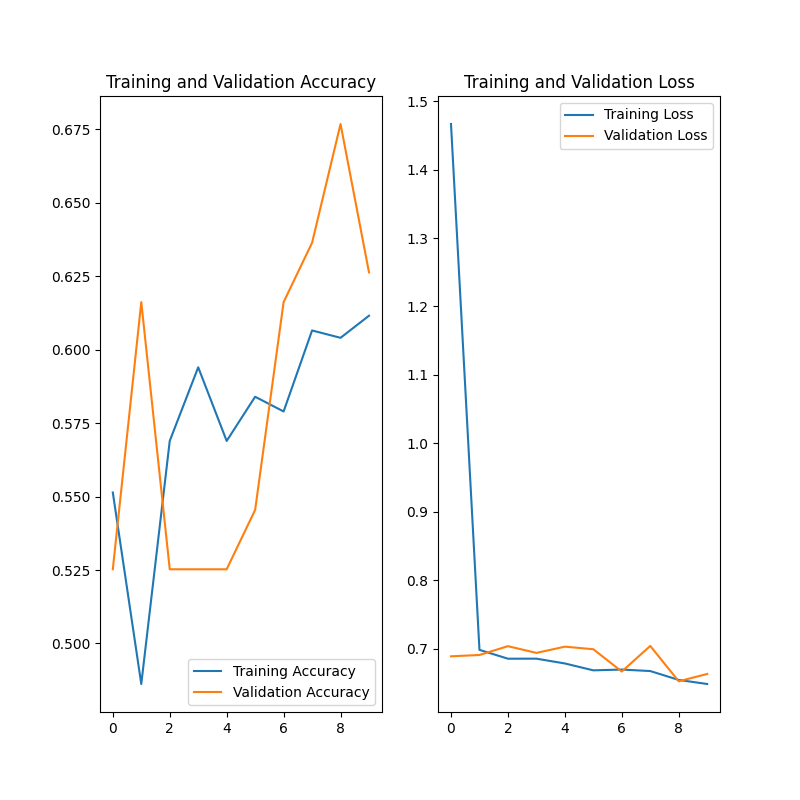
\includegraphics[width=\textwidth]{abbildungen/loss_train_val.png}
        \caption{Mit Data Augmentation}\label{fig:metricsTrainWAugmentation}
    \end{subfigure}
    \caption{Vergleich der Trainings- und Validierungsmetriken mit und ohne Data Augmentation}\label{fig:metricsTrain}
    \textit{Quelle: Eigene Darstellung}
    \\
\end{figure}
Abbildung~\ref{fig:metricsTrain} stellt jeweils die Trainings- und Validierungsmetriken für die \textit{Accuracy} und den \textit{Loss} gegenüber für das Training mit und ohne erweiterte Daten.
Dabei gilt, dass die \textit{Accuracy} gegen eins gehen sollte und der \textit{Loss} gegen null.
Es ist erkennbar, dass die Graphen in beiden Abbildungen relativ früh auseinander gehen, was darauf hindeutet, dass \ldots

Dennoch ist erkennbar, dass die \textit{Data Augmentation} einen klaren Effekt auf den Trainingsverlauf hat. In Abbildung~\ref{fig:metricsTrainWAugmentation} bleiben die Training und Validation Accuracy über alle Epochen hinweg nah beieinander.
In Abbildung~\ref{fig:metricsTrainWOAugmentation} gehen beide Kurven nach der zweiten Epoche auseinander. Dies deutet darauf hin, dass das Modell auf den Trainingsdatensatz overfitted und demnach nicht die richtigen Features der Bilder erlernt.

Insgesamt muss gesagt werden, dass auch mit Data Augmentation die erzielten Genauigkeiten und Losses weit von einem idealen Ergebnis entfernt liegen.
So ist die beste erzielte Genauigkeit mit 67.5\% für ein Klassifizierungsmodell mit lediglich zwei Labeln noch sehr gering und würde wahrscheinlich auf Basis der geringen Menge an Trainingsdaten schlecht generalisieren beziehungsweise auf andere anwendbar sein.

\subsubsection{NER-Modell}
Um den \ac{OSMI}-Index automatisiert bewerten zu können ist es unter anderem notwendig die textbasierten Inhalte einer
Website auf sensorische Inhalte prüfen zu können.
Hierfür eignet sich ein \ac{NER}-Modell, welches die sensorischen Wörter bzw. Begrifflichkeiten als eigene Entität erkennt
am meisten.
Da das Anlernen eines NER-Modells über ein Supervised Learning Verfahren vorgenommen wird, bedarf es einer Datengrundlage,
die vorannotierte Textpassagen enthält auf Basis dessen das Modell trainiert werden kann.
Die Datengrundlage wurde bereits aus vergangenen Projekten durch die Extraktion von Rohtexten der jeweiligen Produktwebseiten
vorgenommen.
Im Rahmen dieses Consulting-Projektes wurden die Rohdaten genutzt, um diese vorzufiltern und anschließend innerhalb von
Doccano zu labeln.
Die gelabelten Textpassagen stellten anschließend die Datengrundlage für das Training des \ac{NER}-Modells dar.
Um es den Annotierern im Vorfeld einfacher zu machen, wurden die Daten vorgefiltert auf mögliche Sensory Words.

Anschließend wurden die annotierten Daten aus Doccano heraus exportiert und in das Trainingsformat für Spacy transformiert.
Das \ac{NER}-Modell wurde im nächsten Schritt auf der Datenbasis trainiert.
Die Ergebnisse des Modelltrainings sind in Abbildung~\ref{fig:NER_Metrics} dargestellt.

\begin{figure}[H]
	\centering
	\caption[]{Ergebnisse des NER-Modell-Trainings}\label{fig:NER_Metrics}
	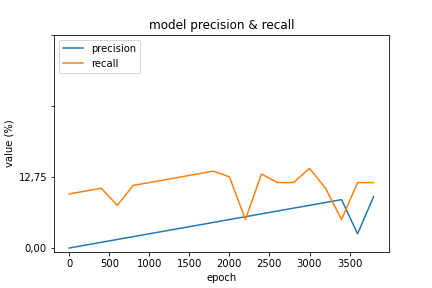
\includegraphics[width=1\textwidth]{NER_Metrics.png}
	\\
	\textit{Quelle: Eigene Darstellung}
\end{figure}

Hier sind die Metriken \textit{Accuracy} und \textit{Recall} je Trainingsepoche abgetragen.
Je besser das Modell trainiert ist, desto mehr nähren sich beide Metriken einem Wert von eins bzw.\ einhundert Prozent an.
Die Abbildung zeigt, dass sowohl die eine als auch die andere Metrik weit vom Optimalwert entfernt sind, was für eine
geringe Modellgüte spricht.

\subsection{Dashboard zur Darstellung der Ergebnisse}\label{subsec_dashboard}
Nachdem das Modell zur Image Classification die relevanten Produktseiten einer Webseite identifiziert hat und das \ac{NER}-Modell
alle relevanten Textpassagen auf die fünf Sinnesentitäten geprüft und diese ausgezählt hat, werden die Ergebnisse
in einem Dashboard ausgegeben und können entsprechend bewertet werden.
Dieses zeigt die Anzahl der erkannten Entitäten aufgeteilt auf die fünf Sinne an und vergleicht diese mit dem Branchendurchschnitt.
Um den jeweiligen Branchendurchschnitt ermitteln zu können, muss vorab eine entsprechende Datenbasis aufgebaut werden,
indem vorab Webseiten wie zu Anfang des Kapitels aufgezeigt durch den Image Classifier selektiert und durch das \ac{NER}-Modell
bewertet werden.
Die Ergebnisse sind jeweils inklusive der Brancheninformationen zu speichern.
Abbildung~\ref{fig:dashboard} zeigt einen möglichen Prototypen, der im Rahmen des Consulting Projektes entwickelt wurde.
\begin{figure}[H]
	\centering
	\caption[]{Dashboard Prototyp}\label{fig:dashboard}
	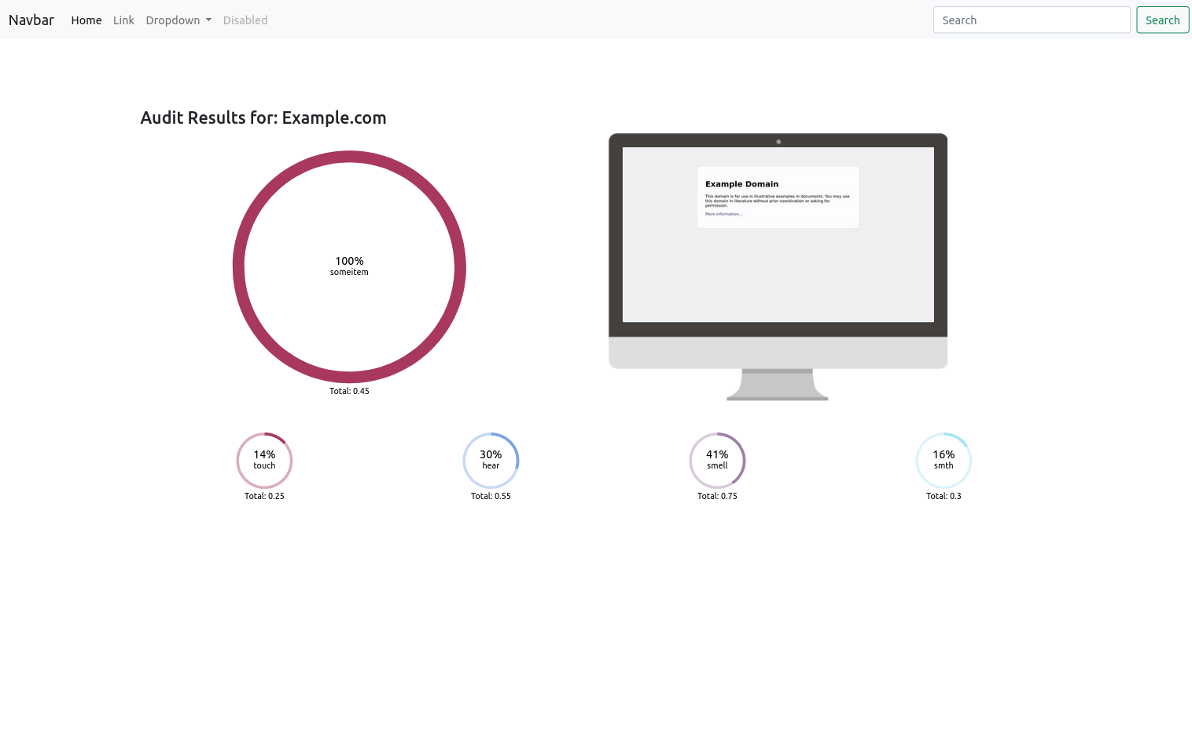
\includegraphics[width=1\textwidth]{dashboard.png}
	\\
	\textit{Quelle: Eigene Darstellung}
\end{figure}

Die kleineren Bewertungen stellen dabei die Ergebnisse der Seite in den einzelnen Sinnesorganen dar. In dem großen Kreis wird das
Resultat des \ac{OSMI}-Index visualisiert.